\documentclass[a4paper,12pt]{article}
\usepackage[left=1.8cm,right=1.8cm,top=2.5cm,bottom=2.5cm]{geometry} % Adjust page margins
\usepackage{xcolor,graphicx,framed}
\usepackage[normalem]{ulem}
\usepackage{amsmath}
\usepackage{cases}
\usepackage{gensymb}
\usepackage{chemmacros}
\setlength{\extrarowheight}{0.4cm}

\begin{document}

\newcommand{\HRule}{\rule{\linewidth}{0.4mm}} % Defines a new command for the horizontal lines, change thickness here

%----------------------------------------------------------------------------------------
%	HEADING SECTIONS
%----------------------------------------------------------------------------------------

\begin{minipage}{0.7\textwidth}
\begin{flushleft} 
\textsc{Universidad del Valle de Guatemala \\
Campus Central \\
Facultad de Ciencias y Humanidades \\
Departamento de Qu\'imica \\
Segundo ciclo, 2014 \\
Fisicoqu\'imica 1 \\
Secci\'on 20
}
\end{flushleft}
\end{minipage}
~
\begin{minipage}{0.2\textwidth}
\begin{flushright}

\includegraphics[scale=0.3]{Logo_UVG} % Include a department/university logo
\end{flushright}
\end{minipage}\\

%----------------------------------------------------------------------------------------
%	TITLE SECTION
%----------------------------------------------------------------------------------------

\begin{center}
\HRule \\[0.4cm]
{ \bfseries Evaluaci\'on 4}\\ % Title of your document
\HRule \\[0.4cm]
\end{center}

%----------------------------------------------------------------------------------------

\section*{Instrucciones}

Responder y resolver los siguientes problemas en las hojas adicionales haciendo uso de regla, calculadora cient\'ifica, una tabla peri\'odica y el formulario individual que haya sido previamente aprobado para su uso. Cualquier actitud deshonesta ser\'a sancionada seg\'un el C\'odigo de comportamiento de los estudiantes de la Universidad.

\section*{Problemas}

\begin{enumerate}

 \item (10 pts) Indicar para cada uno de los siguientes enunciados si es verdadero o falso: % Problema F/V (10 preguntas)
\begin{enumerate}
 \item Si se tiene una soluci\'on ideal para dos componentes, $A$ y $B$, en el equilibrio se cumple que $\mu_A(l)=\mu_B(l)$.
 \item Una soluci\'on ideal no tiene punto eut\'ectico.
 \item El cambio de entalp\'ia cuando mezclo dos gases ideales es $\Delta_{mix}H=0$.
 \item Las propiedades coligativas suceden s\'olo para soluciones dilu\'idas.
 \item En una mezcla binaria de sustancias que no reaccionan entre s\'i, cuando est\'an presentes las fases l\'iquida y vapor, es posible modificar 2 variables independientes sin que cambie el n\'umero de fases.
\end{enumerate}

 \item (15 pts) Dos gramos de \'acido benzoico se disuelven en $25\;\mbox{g}$ de benceno, $K_f=4.90\;\mbox{K}\cdot\mbox{kg}\cdot\mbox{mol}^{-1}$, produciendo una depresi\'on del punto de fusi\'on de $1.62\;\mbox{K}$. Calcular la masa molar del \'acido benzoico. Compararla con la masa molar obtenida a partir de la f\'ormula del \'acido benzoico, $\mbox{C}_6\mbox{H}_5\mbox{COOH}$. % Problema de propiedades coligativas: problema 13.6 de Castellan.

 \item (15 pts) La constante de equilibrio para la siguiente reacci\'on a $25\celsius$:
$$\mbox{CO}_2\mbox{(aq)}+\mbox{H}_2\mbox{O(l)}\;\ch{ <=> }\;\mbox{H}_2\mbox{CO}_3\mbox{(aq)}$$
es $K=2.58\times 10^{-3}$. Si $\Delta_fG^\standardstate(\mbox{CO}_2\mbox{,aq})=-386.0\;\mbox{kJ}\cdot\mbox{mol}^{-1}$ y $\Delta_fG^\standardstate(\mbox{H}_2\mbox{O,l})=-237.18\;\mbox{kJ}\cdot\mbox{mol}^{-1}$, calcular $\Delta_fG^\standardstate(\mbox{H}_2\mbox{CO}_3\mbox{,aq})$. % Problema de equilibrio quimico: problema 14.21 de Castellan.

 \item (15 pts) El entalp\'ia est\'andar de reacci\'on de cierta reacci\'on es aproximadamente constante de $800\;\mbox{K}$ hasta $1500\;\mbox{K}$, teniendo un valor de $+125\;\mbox{kJ}\cdot\mbox{mol}^{-1}$; la energ\'ia de Gibbs est\'andar de reacci\'on es $+22\;\mbox{kJ}\cdot\mbox{mol}^{-1}$ a $1120\;\mbox{K}$. Estimar la temperatura en la cual la constante de equilibrio se convierte mayor a $1$. % Problema de ecuacion de van 't Hoff: problema 6.9(b) de Atkins.

 \item (20 pts) En el laboratorio se trabaj\'o con soluciones entre acetona y cloroformo. El diagrama experimental de temperatura-composici\'on de este sistema a presi\'on constante es el siguiente (en funci\'on de la composici\'on de la acetona):
\begin{center}
 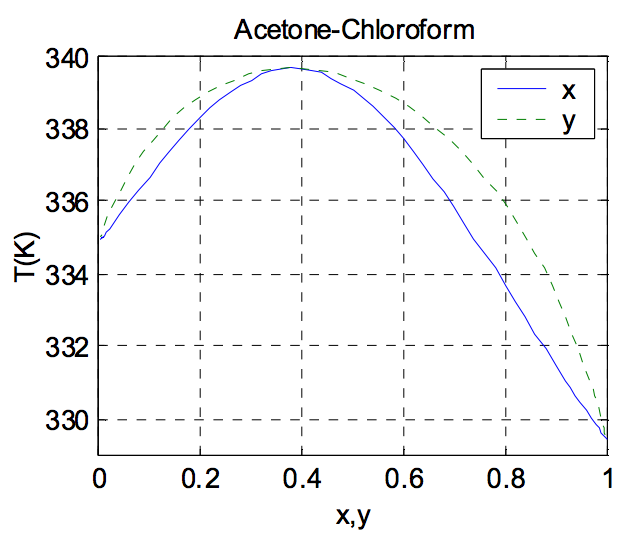
\includegraphics[scale=0.6]{figure4}
\end{center}
\begin{enumerate}
 \item ?`Qu\'e tipo de desviaci\'on con respecto a la ley de Raoult presenta esta soluci\'on?
 \item Se preparan soluciones con fracciones molares del acetona de $0.25$, $0.50$ y $0.75$, y se realiza una destilaci\'on fraccionada para cada una. En cada caso, estimar la temperatura inicial de ebullici\'on, la composici\'on de la primera gota del destilado y la composici\'on de la \'ultima gota en el bal\'on (considerar un n\'umero muy grande de platos te\'oricos).
\end{enumerate} % Problema de interpretar un diagrama de temperatura-composicion.

 \item (25 pts) El benceno y tolueno forman soluciones casi ideales. A $300\;\mbox{K}$, la presiones de vapor del tolueno y benceno son $32.06\;\mbox{mmHg}$ y $103.01\;\mbox{mmHg}$, respectivamente.
\begin{enumerate}
 \item Hacer el diagrama de fase de presi\'on de vapor-composici\'on para el benceno y tolueno a $300\;\mbox{K}$.
 \item Se prepara una muestra l\'iquida con $3\;\mbox{mol}$ de tolueno y $2\;\mbox{mol}$ de benceno. Si la presi\'on exterior es disminuida a $300\;\mbox{K}$, ?`a qu\'e presi\'on comienza a formarse vapor?
 \item ?`Cu\'al es la composici\'on de la primera gota de vapor que se forma?
 \item Si la presi\'on externa se reduce a\'un m\'as, ?`a qu\'e presi\'on desaparece la \'ultima gota del l\'iquido?
 \item ?`Cu\'al es la composici\'on de la \'ultima gota de l\'iquido.
 \item ?`Cu\'al es la presi\'on, la composici\'on del l\'iquido y la composici\'on del vapor cuando $1\;\mbox{mol}$ de mezcla se ha evaporizado? (\emph{Ayuda}: usar la regla de la palanca.)
\end{enumerate} % Problema de hacer un diagrama de presion-composicion: 14.1 de Castellan.

\end{enumerate}

\end{document}
